\documentclass[11pt]{beamer}
\setbeamertemplate{navigation symbols}{}
 \setbeamercovered{transparent}
\usepackage{listings}
%\usetheme{Copenhagen}
\usetheme{Singapore}
%\usetheme{Madrid}
%\usetheme{Hannover}
%\usetheme{boxes}
%\usetheme{Boadilla}
\usefonttheme[onlymath]{serif}
\usecolortheme{beaver}
\usepackage{textpos}
\usepackage{fancyvrb}
\usepackage{xcolor}
\usepackage{multicol}
\usepackage{lipsum}
\parskip 1ex

\newcommand\FontAcolumn{\fontsize{6}{7.2}\selectfont}
\newcommand\FontBcolumn{\fontsize{8}{7.2}\selectfont}
\newcommand\FontCcolumn{\fontsize{10}{7.2}\selectfont}
\newcommand\FontDcolumn{\fontsize{11}{7.2}\selectfont}

\definecolor{gray97}{gray}{.97}
\definecolor{gray75}{gray}{.75}
\definecolor{gray75}{gray}{.45}

\lstdefinestyle{Fortran}{language=[90]Fortran}

\newcommand\FortranStyle
{
\lstset{
frame=Ltb,
framerule=0pt,
columns=fullflexible,
aboveskip=0.5cm,
framextopmargin=3pt,
framexbottommargin=3pt,
framexleftmargin=0.4cm,
framesep=0pt,
rulesep=.4pt,
backgroundcolor=\color{gray97},
rulesepcolor=\color{black},
stringstyle=\ttfamily,
showstringspaces=false,
basicstyle=\ttfamily,
commentstyle=\color{green},
keywordstyle=\color{red},
numbers=left,
numbersep=15pt,
numberstyle=\tiny,
numberfirstline=false,
breaklines=true,
 tabsize=2,
 extendedchars=true,
keepspaces,
}
}

\newcommand\FortranStyleA
{
\lstset{
frame=Ltb,
framerule=0pt,
columns=fullflexible,
aboveskip=0.5cm,
framextopmargin=3pt,
framexbottommargin=3pt,
framexleftmargin=0.4cm,
framesep=0pt,
rulesep=.4pt,
backgroundcolor=\color{gray97},
rulesepcolor=\color{black},
stringstyle=\ttfamily,
showstringspaces=false,
basicstyle=\ttfamily,
commentstyle=\color{green},
keywordstyle=\color{red},
numbersep=15pt,
numberstyle=\tiny,
numberfirstline=false,
breaklines=true,
 tabsize=2,
 extendedchars=true,
keepspaces,
}
}

\newcommand\tab[1][1cm]{\hspace*{#1}}
\newcommand{\light}[1]{\textcolor{lightgray}{#1}}
    
\def\signed #1{{\leavevmode\unskip\nobreak\hfil\penalty50\hskip2em
  \hbox{}\nobreak\hfil(#1)%
  \parfillskip=0pt \finalhyphendemerits=0 \endgraf}}

\newsavebox\mybox
\newenvironment{aquote}[1]
  {\savebox\mybox{#1}\begin{quote}}
  {\signed{\usebox\mybox}\end{quote}}
  
% items enclosed in square brackets are optional; explanation below
\title{An overview of the Fortran programming language}
%\subtitle{Introduction}
\author{Carlos Cruz\\
Jules Kouatchou\\
Bruce Van Aartsen}
\institute{
  NASA GSFC Code 606 (ASTG)\\
  Greenbelt, Maryland 20771\\[1ex]
  \texttt{carlos.a.cruz@nasa.gov}
}
\date{October 24, 2018}

\begin{document}

% --- Title page ---
\begin{frame}[plain]
  \titlepage
\end{frame}

\logo{%
  
\includegraphics[width=1cm,height=1cm,keepaspectratio]{../../shared/nasa-ball.png}%
  \hspace{\dimexpr\paperwidth-2cm-5pt}%
  
\includegraphics[width=1cm,height=1cm,keepaspectratio]{../../shared/ssai-logo.png}%
}

% --- Slide

\begin{frame}{Who we are?}

\begin{itemize}
    \item Carlos A. Cruz (Computational Scientist)
    \item Jules Kouatchou (Computational Scientist)
    \item Bruce Van Aartsen (Senior Software Engineer)
\end{itemize}

\end{frame}

% --- Slide

\begin{frame}{Agenda}

\begin{columns}[onlytextwidth,t]
    \begin{column}{0.48\textwidth}
        \textbf{Day 1}

    \begin{itemize}
        \item Introduction
        \item Variables and data types
        \item Conditionals and loops
        \item Array concepts
        \item Subroutines and functions
        \item Modules and interfaces
        \item File IO
    \end{itemize}
  \end{column}
  \begin{column}{0.48\textwidth}
    \textbf{Day 2}

    \begin{itemize}
        \item Derived types and pointers
        \item Introduction to OOP
        \item IO Enhancements
        \item Inheritance
        \item Polymorphism
        \item Miscellaneous items
        \item Interoperability with C
    \end{itemize}
  \end{column}
\end{columns}

\end{frame}

% --- Slide

\begin{frame}{Agenda}

\textcolor{red}{Introduction}
    \begin{itemize}
        \item History of Fortran
        \item Why Fortran?
        \item Fortran Compilers
        \item Building Projects - Makefile
    \end{itemize}
 
\end{frame}

% --- Slide

\begin{frame}{A Brief History of Fortran}

\begin{itemize}
  \item Origins
  \begin{itemize}
  \scriptsize{
  \item Started ca 1954 by John Backus and his team at IBM
  \item Name comes from \textbf{FOR}mula \textbf{TRAN}slation
  \item First language standard in 1967 (Fortran 66)
  %Fortran 66 was the first ANSI standardized version of the language which made it portable. It introduced common data types, e.g. integer and double precision, block IF and DO statements
  }
  \end{itemize}
  
    \begin{figure}[t]
\centering
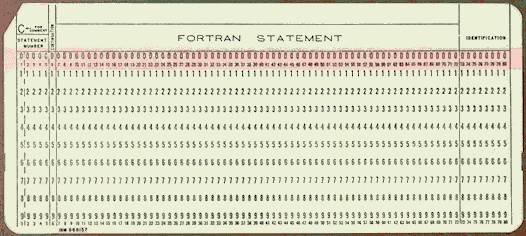
\includegraphics[scale=.3]{../../shared/fortran-card}
\end{figure}

  \item FORTRAN 77
  \begin{itemize}
  \scriptsize{
  \item New standard to overcome divergence in different implementations (1978)
  %Fortran 77 was also another major revision. It introduced file I/O and character data types
  }
  \end{itemize}
  
 
\end{itemize}

\end{frame}

% --- Slide

\begin{frame}{A Brief History of Fortran}

 
  
  \parindent0em


\begin{multicols}{2}[\columnsep2em] 


\begin{itemize}
  \item Fortran 90 (All caps were dropped)
  \begin{itemize}
  \scriptsize{
  \item Major revision. Added modules, derived data types, dynamic memory allocation
  \item Retained backward compatibility
  % Fortran 90 was a major step towards modernizing the language. It allowed free form code, array slicing, modules, interfaces and dynamic memory amongst other features 
  
  }
  \end{itemize}
  
  \item Fortran 95
  \begin{itemize}
  \scriptsize{
  \item Minor revision. Added several HPC related features; forall, where, pure,
  % Fortran 95 was a minor revision which includes pointers, pure and elemental features.
 elemental, pointers
  }
  \end{itemize}
  
    \begin{figure}[t]
\centering
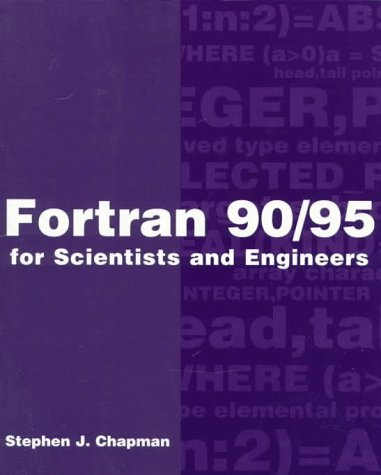
\includegraphics[scale=.3]{../../shared/Fortran-90-95}
\end{figure}
  
  
\end{itemize}


\columnbreak

\end{multicols}



 
\end{frame}

% --- Slide

\begin{frame}{A Brief History of Fortran}



  \parindent0em


\begin{multicols}{2}[\columnsep2em] 

\begin{itemize}
   
  \item Fortran 2003
  \begin{itemize}
  \scriptsize{
  \item Major revision with many new features including; OO capabilities, procedure pointers, IEEE arithmetic, C interoperability
  }
  \end{itemize}
  
  \item Fortran 2008 (latest \emph{stable} release)
  \begin{itemize}
  \scriptsize{
  \item Minor revision. Added co-arrays and submodules  
  }
  \end{itemize}
\end{itemize}

  
    \begin{figure}[t]
\centering
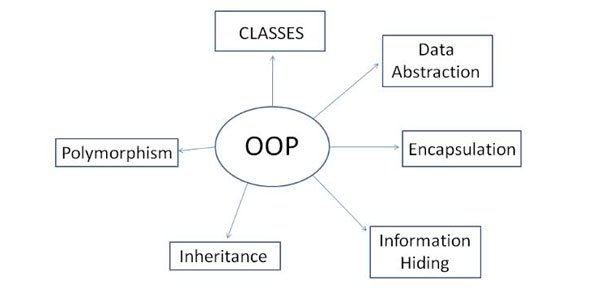
\includegraphics[scale=.25]{../../shared/oop.jpg}
\end{figure}
  
  


\columnbreak

\end{multicols}




\end{frame}

% --- Slide ---
\begin{frame}[fragile]
\frametitle{Why Fortran?}

\begin{itemize}
\item Fortran is the dominant language in HPC applications
 \begin{itemize}
 \item climate/weather models
 \item large scale molecular dynamics
 \item electronic structure calculation codes
 \item modeling of stars and galaxies
 \end{itemize}
 \item Many dense linear algebra libraries developed in Fortran, e.g. BLAS, LAPACK, Scalapack.
 \item Some R and Python linear algebra kernels are written in Fortran.
\end{itemize}

Fortran continues and will continue to be a dominant language for large scale simulation of 
physical systems\footnote{Survey of Fortran users at the 2014 Supercomputing Convention, 100\% of respondents said they thought they would still be using Fortran in five years}.\\

%\scriptsize{
%Reference:\\
%Fortran: The Ideal HPC Programming Language: \url{https://queue.acm.org/detail.cfm?id=1820518}
%}
\end{frame}




% --- Slide

\begin{frame}{Why Fortran?}
% https://arstechnica.com/science/2014/05/scientific-computings-future-can-any-coding-language-top-a-1950s-behemoth/

Unique benefits:
\begin{itemize}

\item Expressiveness / ease
 \begin{itemize}
 \item Arrays lie at the heart of all physics/engineering calculations
 % The array is the most common data structure in computational science.
 \item Little to worry about pointers and memory allocation
 \begin{itemize}
 \item Dynamic arrays in Fortran are not pointers, where in C/C++ they are pointers making them more difficult to deal with.
 \end{itemize}
 \end{itemize}
\item Performance\footnote{Originally proposed as a practical alternative to \textbf{Assembly} language, i.e. it was designed to compete on performance with hand-coded assembler!} 
\item Has added many modern features of programming into newer standards.
\item Legacy code
\item It is \textbf{not} a general purpose programming language like C, C++ and Python.
 \begin{itemize}
 \item It is a language that has been designed exclusively for numerical computation and has applications only in computational science and engineering.
 \end{itemize}
 \end{itemize}

\end{frame}

% --- Slide ---
\begin{frame}[fragile]
\frametitle{}


\centering{
\huge{
Compiling, Linking and Running Fortran Programs
}
}

\end{frame}



% --- Slide ---

\begin{frame}[fragile]
\frametitle{Compilers}

You will need a \textbf{compiler} to produce an executable from Fortran code so that you can...well...execute the program. So, what is a \textbf{compiler}?
\vfill
A compiler is a \textbf{program} that translates source code written in some high-level language - like Fortran - into low-level machine code. The machine code is generally specific to the computer architecture where it was compiled.

% refers to the processing of source code files
%and the creation of an 'object' file
%produces the machine language instructions that correspond to the source code file

\end{frame}



% --- Slide ---

\begin{frame}{Compilation at a glance}

How does a compiler translate source code into executable code?

\begin{figure}[t]
\centering
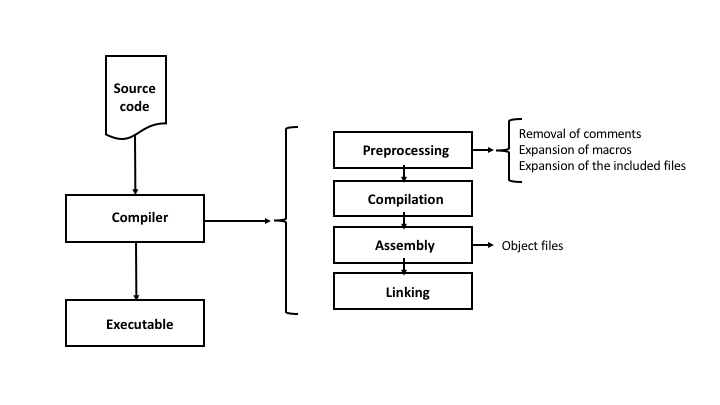
\includegraphics[scale=.3]{../../shared/compiler}
\end{figure}

\end{frame}


\begin{frame}{Some Fortran compiler vendors}

\begin{itemize}
\item \textcolor{red}{GNU}
\item IBM
\item Intel
\item NAG
\item PGI
\end{itemize}

\scriptsize{
\url{https://en.wikipedia.org/wiki/List_of_compilers\#Fortran_compilers}
}

\end{frame}


% --- Slide

%\begin{frame}{Compilation and Linking}
%
%\begin{itemize}
%\item Compilation refers to the processing of source code files and the creation of an 'object' file
%which contains the machine language instructions that correspond to the source code file.
%\begin{itemize}
%\item Compiler errors are usually syntactic in nature.
% \end{itemize}
%
%\item Linking refers to the creation of a single executable file from one or multiple object files
%\begin{itemize}
%\item Linking errors usually have to do with missing or multiple definitions.
% \end{itemize}
%
% \end{itemize}
%
%\end{frame}

% --- Slide

\begin{frame}{The GNU Fortran compiler}

The GNU Fortran compiler supports the Fortran 77, 90 and 95 standards completely, parts
of the Fortran 2003 and Fortran 2008 standards, and several vendor extensions. \\
The GNU Fortran compiler has several components:
\begin{itemize}
\item A version of the \emph{gcc} command that also understands and accepts Fortran source code.
\item The \emph{gfortran} command. The difference with \emph{gcc} is that \emph{gfortran} will automatically link the correct libraries to your program.
\item A collection of run-time libraries. 
\item The Fortran compiler itself, \emph{f951}. \emph{f951} \textbf{translates} the source code to assembler code.
 \end{itemize}
GNU Fortran is a part of GCC, the \emph{GNU Compiler Collection}.

\end{frame}


% --- Slide

\begin{frame}[fragile]
\frametitle{Basic Program Structure}

\FortranStyle

 \begin{lstlisting}[style=Fortran]
PROGRAM program_name $\leftarrow$ stand-alone program
IMPLICIT NONE $\leftarrow$ all variable MUST be declared
! Variable declarations
! ...
! Main program
! ...
STOP $\leftarrow$ stops execution of the program
END PROGRAM
\end{lstlisting}

\end{frame}


% --- Slide

\begin{frame}[fragile]
\frametitle{Hello World!}

\FortranStyle

 \begin{lstlisting}[style=Fortran]
program hello
print *,'Hello World!'
end program
\end{lstlisting}

\end{frame}

% --- Slide ---

\begin{frame}{Using the GNU compiler}

Use \emph{gfortran} command:

\begin{itemize}
\item gfortran hello.F90  $\leftarrow$ no \emph{output} name for the executable specified
\begin{itemize}
\item ./a.out $\leftarrow$ default output file name
\end{itemize}

\item \light{gfortran -c hello.F90 $\leftarrow$ compile only - generates \emph{object} file}
\begin{itemize}
\item \light{hello.o}
\end{itemize}

\item \light{gfortran -c hello.F90 -o hello.o $\leftarrow$  same as previous case}
\begin{itemize}
\item \light{hello.o}
\end{itemize}

\item \light{gfortran -o hello.exe hello.F90 $\leftarrow$  compile and link}
\begin{itemize}
\item \light{./hello.exe}
\end{itemize}

\end{itemize}

\end{frame}

% --- Slide ---

\begin{frame}{Using the GNU compiler}

Use \emph{gfortran} command:

\begin{itemize}
\item \light{gfortran hello.F90  $\leftarrow$ no \emph{output} name for the executable specified}
\begin{itemize}
\item \light{./a.out $\leftarrow$ default output file name}
\end{itemize}

\item gfortran -c hello.F90 $\leftarrow$ compile only - generates \emph{object} file
\begin{itemize}
\item hello.o
\end{itemize}

\item gfortran -c hello.F90 -o hello.o $\leftarrow$  same as previous case
\begin{itemize}
\item hello.o
\end{itemize}

\item \light{gfortran -o hello.exe hello.F90 $\leftarrow$  compile and link}
\begin{itemize}
\item \light{./hello.exe}
\end{itemize}

\end{itemize}

\end{frame}


% --- Slide ---

\begin{frame}{Using the GNU compiler}

Use \emph{gfortran} command:

\begin{itemize}
\item \light{gfortran hello.F90  $\leftarrow$ no \emph{output} name for the executable specified}
\begin{itemize}
\item \light{./a.out $\leftarrow$ default output file name}
\end{itemize}

\item \light{gfortran -c hello.F90 $\leftarrow$ compile only - generates \emph{object} file}
\begin{itemize}
\item \light{hello.o}
\end{itemize}

\item \light{gfortran -c hello.F90 -o hello.o $\leftarrow$  same as previous case}
\begin{itemize}
\item \light{hello.o}
\end{itemize}

\item gfortran -o hello.exe hello.F90 $\leftarrow$  compile and link
\begin{itemize}
\item ./hello.exe
\end{itemize}

\end{itemize}

\end{frame}

% --- Slide ---

\begin{frame}[fragile]
\frametitle{Libraries}

After compilation we generally want to create a \emph{static} library. For that we use the program�"ar"�(stands for archiver) as follows:
\begin{Verbatim} 
$ gfortran -c *.F90
$ ar -r libmystatlib.a *.o
\end{Verbatim}
one can also create a \emph{dynamic} library...
\begin{Verbatim}
$ gfortran -c -fPIC *.F90  
$ gfortran -shared -o libmydynlib.so *.o
\end{Verbatim}

\end{frame}



% --- Slide ---

\begin{frame}[fragile]
\frametitle{Linking}

A linker takes several object files and libraries as input and produces one executable object file. Additionally,
\begin{itemize}
\item it resolves all external references
\item it includes the operating system libraries, the language-specific libraries, and, maybe, user-created libraries. 
\end{itemize}

\end{frame}




%% --- Slide ---
%
%\begin{frame}[fragile]
%\frametitle{Linking libraries}
%
%\begin{itemize}
%\item Static and dynamic linking
%\begin{itemize}
%\item Static - performed by linker
%\item Dynamic - performed by OS
%\end{itemize}
%\end{itemize}
%
%\end{frame}

% --- Slide ---

\begin{frame}[fragile]
\frametitle{make}
What is \textbf{make}?
\begin{itemize}
\item The \textbf{make} utility is a tool for managing and maintaining computer programs. It is generally used to build executable programs, libraries, and other files.
\item Created at Bell Labs ca. 1977 
\item The input to make is a file called the \textbf{makefile}.
\item The \textbf{makefile}  describes a set of targets, which are the objects that can be \textbf{made}.
\item \textbf{make} is programming language agnostic.
\item \textbf{make} is one of the most essential tools for programmers.
\end{itemize}
Reference: \url{http://www.gnu.org/software/make/}

\end{frame}

% Make is the de-facto tool for building executable programs from source code in the world of open source.
% Make enables end users to build executable programs without knowing technical details of how to build them

% --- Slide ---

\begin{frame}[fragile]
\frametitle{The makefile}

\scriptsize{
The \textbf{makefile} is a collection of \emph{rules}. 
\begin{itemize}
\item The rules instruct \textbf{make} how to build a target 
\item A rule also specifies dependencies of the target. 
\end{itemize}
The dependency rules must be executed first depending on whether that is already 
processed by looking at the time stamps.\\
\vspace{5mm}
Rule syntax:\\
\vspace{5mm}
\emph{target}: \emph{dependencies}\quad \quad $\leftarrow$ AKA a \emph{prerequisite}\\
\tab \emph{commands}\\
\quad $\uparrow$\\
Tab
}
\end{frame}

%The beauty of Make is that it?s simply a rigorous way of recording what you?re already doing. It doesn?t fundamentally change how you do something, but it encourages to you record each step in the process, enabling you (and your coworkers) to reproduce the entire process later.

%The core concept is that generated files depend on other files. When generated files are missing, or when files they depend on have changed, needed files are re-made using a sequence of commands you specify. 


% --- Slide ---

\begin{frame}[fragile]
\frametitle{The makefile}
\begin{itemize}
\item Standard names: makefile, Makefile, GNUmakefile.
\item To run:
\begin{Verbatim}
$ make  
$ make some_target
\end{Verbatim}
\item If using a non-standard name, say my\_app.make
\begin{Verbatim}
$ make -f my_app.make
\end{Verbatim}
\end{itemize}

\end{frame}


% --- Slide ---

\begin{frame}[fragile]
\frametitle{The makefile}

\footnotesize{
\begin{Verbatim}[frame=single]
hello.exe: hello.o
        gfortran hello.o -o hello.exe 
        
hello.o: hello.F90
        gfortran -c hello.F90
clean:
	rm *.o *.exe
\end{Verbatim}

\begin{verbatim}
$ make  (or make hello.exe)
gfortran -o hello.exe hello.F90 -I.
$ ls
GNUmakefile  hello.exe  hello.F90
$ ./hello.exe
 hello world!
\end{verbatim}
}

\end{frame}


% --- Slide

\begin{frame}[fragile]
\frametitle{Conclusion}

References:
\scriptsize{
\begin{itemize}
\item \url{https://gcc.gnu.org/fortran/}
\item \url{http://fortranwiki.org/fortran/show/HomePage}
\item \url{https://en.wikipedia.org/wiki/Fortran}
\item \url{https://www.gnu.org/software/make/manual/make.html}
\end{itemize}
}

\end{frame}

\end{document}
